\documentclass[12pt,a4paper]{article}
\usepackage[utf8]{inputenc} % inutile avec XeLaTeX/LuaLaTeX
\usepackage[T1]{fontenc}
\usepackage{amsmath,amssymb,mathrsfs,tikz,times,pifont}
\usepackage{enumitem}
\usepackage{multicol}
\usepackage{lmodern}
\newcommand\circitem[1]{%
\tikz[baseline=(char.base)]{
\node[circle,draw=gray, fill=red!55,
minimum size=1.2em,inner sep=0] (char) {#1};}}
\newcommand\boxitem[1]{%
\tikz[baseline=(char.base)]{
\node[fill=cyan,
minimum size=1.2em,inner sep=0] (char) {#1};}}
\setlist[enumerate,1]{label=\protect\circitem{\arabic*}}
\setlist[enumerate,2]{label=\protect\boxitem{\alph*}}
\everymath{\displaystyle}
\usepackage[left=1cm,right=1cm,top=1cm,bottom=1.7cm]{geometry}
\usepackage[colorlinks=true, linkcolor=blue, urlcolor=blue, citecolor=blue]{hyperref}
\usepackage{array,multirow}
\usepackage[most]{tcolorbox}
\usepackage{varwidth}
\usepackage{float}
\tcbuselibrary{skins,hooks}
\usetikzlibrary{patterns}

\newtcolorbox{exa}[2][]{enhanced,breakable,before skip=2mm,after skip=5mm,
colback=yellow!20!white,colframe=black!20!blue,boxrule=0.5mm,
attach boxed title to top left ={xshift=0.6cm,yshift*=1mm-\tcboxedtitleheight},
fonttitle=\bfseries,
title={#2},#1,
boxed title style={frame code={
\path[fill=tcbcolback!30!black]
([yshift=-1mm,xshift=-1mm]frame.north west)
arc[start angle=0,end angle=180,radius=1mm]
([yshift=-1mm,xshift=1mm]frame.north east)
arc[start angle=180,end angle=0,radius=1mm];
\path[left color=tcbcolback!60!black,right color = tcbcolback!60!black,
middle color = tcbcolback!80!black]
([xshift=-2mm]frame.north west) -- ([xshift=2mm]frame.north east)
[rounded corners=1mm]-- ([xshift=1mm,yshift=-1mm]frame.north east)
-- (frame.south east) -- (frame.south west)
-- ([xshift=-1mm,yshift=-1mm]frame.north west)
[sharp corners]-- cycle;
},interior engine=empty,
},interior style={top color=yellow!5}}

\usepackage{fancyhdr}
\usepackage{eso-pic}
\usepackage{tkz-tab}
\AddToShipoutPicture{
    \AtTextCenter{%
        \makebox[0pt]{\rotatebox{80}{\textcolor[gray]{0.7}{\fontsize{5cm}{5cm}\selectfont PGB}}}
    }
}

\usepackage{verbatim}

\usepackage{color,soul}

\usepackage{amsmath}
\usepackage{amsfonts}
\usepackage{amssymb}
\usepackage{systeme}
\usepackage{tkz-tab}
\usepackage{tikz}
\usetikzlibrary{calc}
\usetikzlibrary{arrows}
\newcounter{exemple} % Compteur pour les questions

% Définir la commande pour afficher une question numérotée
\newcommand{\exemple}{%
  \refstepcounter{exemple}%
  \textbf{\textcolor{green}{Exemple \theexemple :}} \ignorespaces
}
%---------------------------------------
%\definecolor{myorange}{rgb}{1.0, 0.8, 0.0}

% Définir un compteur pour les exercices d'application
\newcounter{exerciceapp}

% Définir la commande pour afficher un exercice d'application numéroté
\newcommand{\exerciceapp}{%
  \refstepcounter{exerciceapp}%
  \textbf{\textcolor{green}{Exercice d'application \theexerciceapp :}} \ignorespaces
}
%--------------------------------------
% Définir un compteur pour les exercices d'application
\newcounter{correction}

% Définir la commande pour afficher un correction exercice d'application numéroté
\newcommand{\correction}{%
  \refstepcounter{correction}%
  \textbf{\textcolor{green}{Correction \thecorrection :}} \ignorespaces
}
%--------------------------------------
% Commande pour ajouter du texte en arrière-plan
\usepackage{fancyhdr}
\usepackage{eso-pic}
%\usepackage{tkz-tab}
\AddToShipoutPicture{
    \AtTextCenter{%
        \makebox[0pt]{\rotatebox{80}{\textcolor[gray]{0.7}{\fontsize{5cm}{5cm}\selectfont PGB}}}
    }
}
%This command takes a colour as an optional argument; the default colour is black.
\usetikzlibrary{shapes.geometric,fit}
\newcommand{\myul}[2][black]{\setulcolor{#1}\ul{#2}\setulcolor{black}}
\newcommand\tab[1][1cm]{\hspace*{#1}}

\begin{document}
% En-tête personnalisée
\begin{center}
    \Large\textbf{\underline{Droites Remarquables Dans Un Triangle}}\\[0.2cm]
    \normalsize\textbf{Prof : M. BA} \hfill \textbf{Classe : 4eme}\\[0.1cm]
    \textbf{Année scolaire : 2025 -- 2026}
\end{center}

\begin{center}
\textbf{Introduction}
\end{center}



\section*{\underline{\textbf{\textcolor{red}{I. Bissectrices d’un triangle :}}}}

\paragraph{\textcolor{red}{1) \underline{Définition} :}}
Une bissectrice d'un triangle est une droite qui passe par le sommet d'un angle de ce triangle et qui partage cet angle en deux angles égaux.

\paragraph{\textcolor{red}{2) \underline{Méthode} :}}

Pour construire la bissectrice d'un angle $\widehat{BAC}$ d'un triangle $ABC$, il faut :
\begin{itemize}
    \item[$\checkmark$] Construire un triangle $ABC$,
    \item[$\checkmark$] Construire un arc de cercle qui coupe $[AB)$ en $E$ et $[AC)$ en $F$,
    \item[$\checkmark$] Construire deux arcs de cercle de même rayon sécants en $G$, l'un de centre $E$ et l'autre de centre $F$,
    \item[$\checkmark$] La droite $(AG)$ est la bissectrice de l'angle $\widehat{BAC}$.
\end{itemize}

% --- Début de la figure TikZ ---
\begin{center}
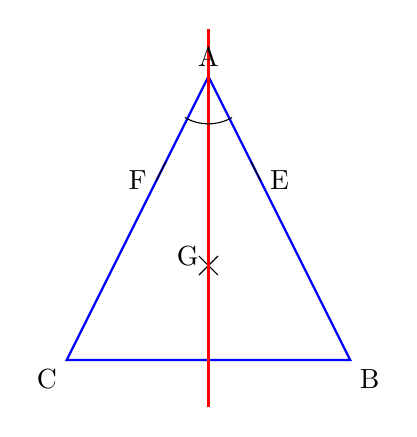
\begin{tikzpicture}[scale=1.2]
    % Définition des points
    \coordinate (A) at (0,3);
    \coordinate (B) at (1.5,0);
    \coordinate (C) at (-1.5,0);
    
    % Dessin du triangle
    \draw[thick, blue] (A) -- (B) -- (C) -- cycle;
    
    % Points E et F (intersection arc de cercle)
    \coordinate (E) at (0.5,2);
    \coordinate (F) at (-0.5,2);
    
    % Marques E et F
    \draw (0.45,2.1) -- (0.55,1.9) node[right] {E};
    \draw (-0.45,2.1) -- (-0.55,1.9) node[left] {F};
    
    % Point G et son intersection
    \coordinate (G) at (0,1);
    \draw (-0.1,1.1) -- (0.1,0.9);
    \draw (0.1,1.1) -- (-0.1,0.9);
    \node[left] at (0,1.1) {G};
    
    % La bissectrice en rouge
    \draw[very thick, red] (0,3.5) -- (0,-0.5);
    
    % Marquage des angles égaux
    \draw (0,2.5) arc (270:300:0.5);
    \draw (0,2.5) arc (270:240:0.5);
    
    % Noms des sommets
    \node[above] at (A) {A};
    \node[below right] at (B) {B};
    \node[below left] at (C) {C};
\end{tikzpicture}
\end{center}
% --- Fin de la figure TikZ ---

\paragraph{\textcolor{red}{3) \underline{Propriétés} :}}
\begin{itemize}
    \item[$\checkmark$] Si un point appartient à la bissectrice d'un angle, alors il est équidistant des côtés de cet angle.
    \item[$\checkmark$] Les trois bissectrices d'un triangle sont concourantes.
\end{itemize}

\paragraph{\textcolor{red}{4) \underline{Cercle inscrit dans un triangle} :}}

\subparagraph{\textcolor{red}{a) \underline{Vocabulaire} :}}
\begin{itemize}
    \item[$\checkmark$] Le point de concours de ces trois bissectrices est le centre du cercle tangent aux trois côtés du triangle.
    \item[$\checkmark$] Ce cercle est appelé cercle inscrit dans le triangle et tangent à chacun des côtés de ce triangle.
\end{itemize}

\subparagraph{\textcolor{red}{b) \underline{Méthode de construction} :}}
Pour tracer le cercle inscrit dans un triangle, il faut :
\begin{itemize}
    \item[$\checkmark$] Tracer soigneusement deux bissectrices de ce triangle,
    \item[$\checkmark$] Construire le projeté orthogonal H de leur point d'intersection I sur un des côtés du triangle.
    \item[$\checkmark$] Tracer le cercle de centre I et de rayon IH.
\end{itemize}

% --- Début de la figure TikZ ---
\begin{center}
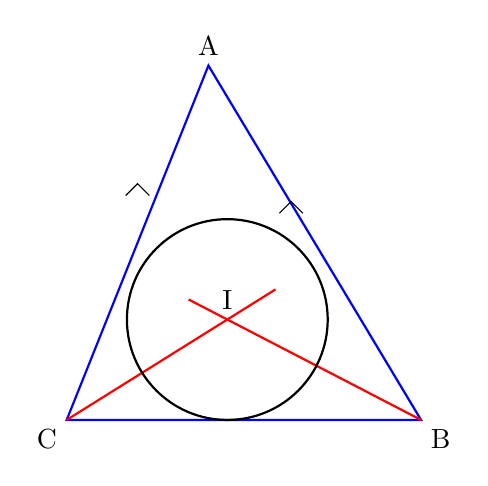
\begin{tikzpicture}[scale=1.5]
    % Coordonnées des sommets du triangle
    \coordinate (A) at (0,3);
    \coordinate (B) at (1.8,0);
    \coordinate (C) at (-1.2,0);
    
    % Dessin du triangle
    \draw[thick, blue] (A) -- (B) -- (C) -- cycle;
    
    % Calcul du centre du cercle inscrit (Incenter)
    % Formule simplifiée pour ce triangle spécifique
    \coordinate (I) at (0.16,0.85); 
    
    % Dessin des bissectrices en rouge
    % Bissectrice partant de C
    \draw[thick, red] (C) -- ($(C)!1.3!(I)$);
    % Bissectrice partant de B
    \draw[thick, red] (B) -- ($(B)!1.2!(I)$);
    
    % Projection orthogonale (H) sur le côté AB pour illustration
    % (Approximation visuelle pour coller au schéma)
    \coordinate (H) at (0.8, 1.65);
    
    % Dessin du cercle inscrit
    \draw[thick] (I) circle (0.85cm);
    
    % Labels
    \node[above] at (A) {A};
    \node[below right] at (B) {B};
    \node[below left] at (C) {C};
    \node[above] at (I) {I};
    
    % Symboles d'angle droit (projections orthogonales)
    \draw (0.6, 1.75) -- (0.7, 1.85) -- (0.8, 1.75);
    \draw (-0.5, 1.9) -- (-0.6, 2.0) -- (-0.7, 1.9);
    
\end{tikzpicture}
\end{center}
% --- Fin de la figure TikZ ---
\textbf{\exerciceapp}

\textbf{\correction}
\section*{\underline{\textbf{\textcolor{red}{I. Médianes d’un triangle :}}}}
\subsection*{\underline{\textbf{\textcolor{red}{1) Définition :}}}}

Une médiane d’un triangle est une droite qui passe par un sommet et par le milieu du côté opposé à ce sommet.

\subsection*{\underline{\textbf{\textcolor{red}{2) Propriétés :}}}}

\begin{itemize}
\item[$\checkmark$] Les trois médianes d’un triangle sont concourantes.
\item[$\checkmark$] Le point de concours de ces médianes est appelé centre de gravité du triangle.
\item[$\checkmark$] Le centre de gravité d’un triangle se trouve au deux tiers de chaque médiane à partir du sommet.
\end{itemize}
\textbf{\exerciceapp}

\textbf{\correction}

\section*{\underline{\textbf{\textcolor{red}{I. Médiatrices d’un triangle :}}}}
\subsection*{\underline{\textbf{\textcolor{red}{1) Définition :}}}}
Une médiatrice d’un triangle est une droite qui passe par le milieu d’un coté et perpendiculaire à ce coté.
\subsection*{\underline{\textbf{\textcolor{red}{2) Propriétés :}}}}

\begin{itemize}
\item[$\checkmark$] Les trois médiatrices d’un triangle sont concourantes.
\item[$\checkmark$] Leur point de concours est le centre du cercle passant par les trois sommets du triangle.
\item[$\checkmark$] Ce cercle est appelé cercle circonscrit au triangle.
\end{itemize}

\textbf{\underline{\textbf{\textcolor{red}{ Remarques :}}}}
\begin{itemize}
\item[$\checkmark$] Quand le triangle a trois angles aigus, le centre du cercle circonscrit est à l’intérieur du triangle.
\item[$\checkmark$] Quand le triangle a un angle obtus, le centre du cercle circonscrit est à l’extérieur du triangle.
\item[$\checkmark$] Quand le triangle a un angle droit, le centre du cercle circonscrit est le milieu de l’hypoténuse.
\end{itemize}

\textbf{\underline{\textbf{\textcolor{red}{ Remarques :}}}}

\textbf{\exerciceapp}

\textbf{\correction}

\section*{\underline{\textbf{\textcolor{red}{I. Hauteurs d’un triangle :}}}}
\subsection*{\underline{\textbf{\textcolor{red}{1) Définition :}}}}
Une hauteur d’un triangle est une droite qui passe par un sommet du triangle et qui est perpendiculaire au coté
opposé à ce sommet.
\subsection*{\underline{\textbf{\textcolor{red}{2) Propriétés :}}}}

\begin{itemize}
\item[$\checkmark$] Les trois hauteurs d’un triangle sont concourantes.
\item[$\checkmark$] Le point de concours de ces trois hauteurs est appelé orthocentre du triangle.
\end{itemize}

\textbf{\underline{\textbf{\textcolor{red}{ Remarques :}}}}



\begin{itemize}
\item[$\checkmark$] Si un triangle a un angle obtus, l’orthocentre est à l’extérieur.
\item[$\checkmark$] Si un triangle est rectangle, l’orthocentre est le sommet de l’angle droit.
\item[$\checkmark$] Si les angles sont aigus, l’orthocentre est à l’intérieur du triangle.
\end{itemize}
\textbf{\exerciceapp}

\textbf{\correction}

\section*{\underline{\textbf{\textcolor{red}{V. Reconnaissance d’un triangle isocèle :}}}}

\textbf{\underline{\textbf{\textcolor{red}{ Remarques :}}}}

\underline{\exemple}
\end{document}
